%!TEX root = ../../book_ML.tex
\chapter{Hệ thống gợi ý dựa trên nội dung}
% \chapter{Content-based recommendation system}

\index{hệ thống gợi ý -- recommendation system!}
\index{hệ thống gợi ý -- recommendation system! dựa trên nội dung -- content-based}
 
\section{Giới thiệu}
\index{hệ thống gợi ý -- recommendation system! người dùng}
\index{hệ thống gợi ý -- recommendation system! sản phẩm}
Hệ thống gợi ý là một mảng khá rộng của machine learning và có
xuất hiện sau phân loại hay hồi quy vì internet mới
chỉ thực sự bùng nổ khoảng 10-15 năm gần đây. Có hai thực thể chính trong một
hệ thống gợi ý là \textit{người dùng} (user) và \textit{sản phẩm} (item). Mục đích chính của các hệ thống gợi ý là dự đoán mức độ quan tâm của một người dùng tới một sản phẩm nào đó, qua đó có chiến lược gợi ý phù hợp. 
% Để thống nhất với các ký hiệu toán học và h
 
 
\subsection{Hiện tượng \textit{đuôi dài}}
\index{hệ thống gợi ý -- recommendation system! hiện tượng đuôi dài -- long tail}

Chúng ta cùng đi vào việc so sánh điểm khác nhau căn bản giữa các {cửa
hàng thực} và {cửa hàng điện tử} trên khía cạnh lựa chọn sản
phẩm để quảng bá. {Ở đây, chúng ta tạm quên đi khía cạnh {cảm giác
thật chạm vào sản phẩm} của các cửa hàng thực và tập trung vào phần làm
thế nào để quảng bá đúng sản phẩm tới khách hàng.}
 
Có thể các bạn đã biết tới \textit{Nguyên lý Pareto} (quy tắc 20/80)
(\url{https://goo.gl/NujWjH}): \textit{phần lớn kết quả được gây ra bởi phần nhỏ
nguyên nhân}. Phần lớn số từ sử dụng hàng ngày chỉ là một phần nhỏ trong
từ điển. Phần lớn của cải được sở hữu bởi phần nhỏ số người. Trong hương
mại, những sản phẩm bán chạy nhất chiếm phần nhỏ trên tổng số sản phẩm.
 
Các {cửa hàng thực} thường có hai khu vực: khu trưng bày và kho. Nguyên tắc dễ thấy để đạt doanh thu cao là trưng ra các sản phẩm phổ biến ở những nơi dễ thấy nhất và cất những sản phẩm ít phổ biến hơn trong kho. Cách
làm này có một hạn chế rõ rệt: những sản phẩm được trưng ra mang tính phổ biến
nhưng chưa chắc đã phù hợp với nhu cầu của một khách hàng cụ thể. Một cửa hàng có thể có món hàng một người đang tìm kiếm nhưng không bán được vì khách hàng đó không tìm thấy sản phẩm. Điều này dẫn đến việc khách hàng không tiếp cận
được sản phẩm ngay cả khi chúng đã được trưng ra. Ngoài ra, vì không gian có
hạn, cửa hàng không thể trưng ra tất cả các sản phẩm mà mỗi loại chỉ đưa ra một
số lượng nhỏ. Ở đây, phần lớn doanh thu (80\%) đến từ phần nhỏ số sản phẩm phổ
biến nhất (20\%). Nếu sắp xếp các sản phẩm của cửa hàng theo doanh số từ cao đến
thấp, ta sẽ nhận thấy có thể phần nhỏ các sản phẩm tạo ra phần lớn doanh số. Và
một danh sách dài phía sau chỉ đóng góp một lượng nhỏ. Hiện tượng này còn
được gọi là \textit{đuôi dài} (long tail phenomenon).
 
Với các {cửa hàng điện tử}, nhược điểm trên hoàn toàn có thể tránh được vì {gian trưng bày} của các {cửa hàng điện tử} gần như là vô tận,
mọi sản phẩm đều có thể được trưng ra. Hơn nữa, việc sắp xếp online là linh
hoạt, tiện lợi với chi phí chuyển đổi gần như bằng không khiến việc mang đúng sản
phẩm tới khách hàng trở nên thuận tiện. Doanh thu vì thế có thể được tăng
lên.
 

 
 
 
\subsection{Hai nhóm thuật toán trong hệ thống gợi ý}
\index{hệ thống gợi ý -- recommendation system! lọc cộng tác -- collaborative filtering}
Các thuật toán trong hệ thống gợi ý được chia thành hai nhóm lớn: 
\begin{enumerate}
    \item \textit{Hệ thống dựa trên nội dung}: Gợi ý dựa trên đặc tính của sản
    phẩm. Ví dụ, hệ thống nên gợi ý các bộ phim hình sự tới những người thích xem phim ``Cảnh sát hình sự'' hay ``Người phán xử''. Cách tiếp cận này
    yêu cầu sắp xếp các sản phẩm vào từng nhóm hoặc đi tìm các đặc
    trưng của từng sản phẩm. Tuy nhiên, có những sản phẩm không có
    rơi vào một nhóm cụ thể và việc xác định nhóm hoặc đặc trưng của từng sản phẩm đôi khi bất khả thi.
     
     
    \item \textit{Lọc cộng tác} (collaborative filtering): Hệ thống gợi ý các
    sản phẩm dựa trên sự tương quan giữa người dùng và/hoặc sản phẩm. Ở nhóm
    này, một sản phẩm được {gợi ý} tới một người dùng dựa trên những người dùng
    có sở thích tương tự hoặc những sản phẩm tương ựu. Ví dụ, ba người dùng ${A,
    B, C}$ đều thích các bài hát của Noo Phước Thịnh. Ngoài ra, hệ thống biết
    rằng người dùng \textit{B, C} cũng thích các bài hát của Bích Phương nhưng
    chưa có thông tin về việc liệu người dùng \textit{A} có thích ca sĩ này hay
    không. Dựa trên thông tin của những người dùng tương tự là \textit{B và C},
    hệ thống có thể dự đoán rằng \textit{A} cũng thích Bích Phương và gợi ý các
    bài hát của ca sĩ này tới \textit{A}.
 
\end{enumerate}
Trong chương này, chúng ta sẽ làm quen với nhóm thuật toán thứ nhất. Nhóm thuật toán thứ hai, lọc cộng tác, sẽ được trình bày trong
các chương tiếp theo.

% Các từ \textit{người dùng} và \textit{sản phẩm} từ đây sẽ được thay thế bởi
% \textit{user} và sản phẩm để có sự thống nhất giữa một số tên gọi và các
% ký hiệu toán học. 
\section{Ma trận tiện ích}
\index{hệ thống gợi ý -- recommendation system! ma trận tiện ích -- utility matrix}
Có hai thực thể chính trong các hệ thống gợi ý là
\textit{người dùng} và \textit{sản phẩm}. Mỗi người dùng có mức quan tâm tới từng sản phẩm khác nhau. Thông tin về mức độ quan tâm của một người dùng tới một
sản phẩm có thể được thu thập thông qua một hệ thống đánh
giá ({review} và {rating}), qua việc người dùng đã click vào thông tin
của sản phẩm hoặc qua thời lượng người dùng xem thông tin của một sản phẩm. Các ví dụ trong phần này đều dựa trên hệ thống đánh giá sản phẩm.

\subsection{Ma trận tiện ích}

\begin{figure}[t]
    % caption on side     
    \floatbox[{\capbeside\thisfloatsetup{capbesideposition={right,top},capbesidewidth=6cm}}]{figure}[\FBwidth]
    {\caption{ 
    Ví dụ về ma trận tiện ích với hệ thống gợi ý bài hát. Các bài hát được người dùng đánh giá theo mức độ từ 0
    đến 5 sao. Các dấu '?' nền màu xám ứng với việc dữ liệu còn thiếu. Hệ thống gợi ý cần dự đoán các giá trị này.
    }
    \label{fig:23_1}}
    { % figure here
    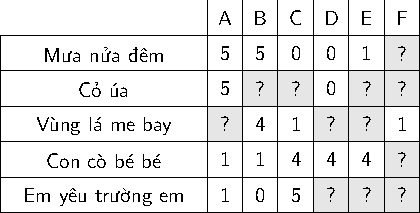
\includegraphics[width=.5\textwidth]{Chapters/06_RecommendationSystems/23_contentbasedrecommendersys/latex/utility1.pdf}
    }
\end{figure}
 
\index{hoàn thiện ma trận -- matrix completion}
Với một hệ thống đánh giá sản phẩm, {mức độ quan tâm} của một người dùng
tới một sản phẩm được đo bằng số sao trên tổng số sao, chẳng hạn năm sao. Tập hợp tất cả các đánh giá ở dạng số, bao gồm cả những giá trị cần được dự đoán, tạo nên
một ma trận gọi là \textit{ma trận tiện ích} (utility matrix). Xét ví dụ trong
Hình~\ref{fig:23_1}, có sáu người dùng \textit{A, B, C, D, E, F} và
năm bài hát. Các ô đã được đánh số thể hiện việc một người dùng đã đánh giá
một bài hát từ 0 (không thích) đến 5 (rất thích). Các ô có
dấu '?' tương ứng với các ô chưa có dữ liệu. Công việc của một
hệ thống gợi ý là dự đoán giá trị tại các ô màu xám này, từ đó đưa ra gợi
ý cho người dùng. Vì vậy, bài toán hệ thống gợi ý đôi khi được coi là
bài toán \textit{hoàn thiện ma trận} ({matrix completion}).
 
Nhận thấy có hai thể loại nhạc khác nhau: ba bài
đầu là nhạc {bolero} và hai bài sau là nhạc {thiếu nhi}. Từ dữ
liệu này, ta cũng có thể đoán được rằng \textit{A, B} thích thể loại nhạc
{Bolero}; trong khi \textit{C, D, E, F} thích nhạc {thiếu
nhi}. Từ đó, một hệ thống tốt nên gợi ý ``{Cỏ úa}'' cho \textit{B};
``{Vùng lá me bay}'' cho \textit{A}; ``{Em yêu trường em}'' cho \textit{D,
E, F}. Giả sử chỉ có hai thể loại nhạc này, khi có một bài hát mới, ta cần
phân loại rồi đưa ra gợi ý với từng người dùng.
 
Thông thường, có rất nhiều người dùng và sản phẩm trong hệ thống nhưng mỗi
người dùng chỉ đánh giá một lượng nhỏ các sản phẩm,
thậm chí có những người dùng không đánh giá sản phẩm nào. Vì vậy, lượng ô
màu xám của ma trận tiện ích thường rất lớn so với lượng ô màu trắng đã biết. 

Rõ ràng, càng nhiều ô được điền thì độ chính xác của hệ thống sẽ càng được cải
thiện. Vì vậy, các hệ thống luôn khuyến khích người dùng {bày tỏ} sự quan tâm
của họ tới các sản phẩm thông qua việc đánh giá các sản phẩm đó. Việc đánh giá
không những giúp người dùng khác biết được chất lượng của sản phẩm mà còn giúp
hệ thống {biết} được sở thích của người dùng, qua đó có chính sách quảng cáo hợp
lý.
 
 
\subsection{Xây dựng ma trận tiện ích}
 
Không có ma trận tiện ích, hệ thống gần như không thể gợi ý được sản phẩm tới
người dùng. Vì vậy, việc xây dựng ma trận tiện ích là tối quan trọng trong các
hệ thống gợi ý. Tuy nhiên, việc xây dựng ma trận này thường gặp nhiều khó khăn.
Có hai hướng tiếp cận phổ biến để xác định giá trị đánh giá cho mỗi cặp (người
dùng, sản phẩm) trong ma trận tiện ích:
\vspace{-0.25cm}
\begin{enumerate}
    \item Khuyến khích người dùng đánh giá sản phẩm. Amazon luôn
    khuyến khích người dùng đánh giá các sản phẩm bằng cách gửi mail nhắc nhở
    nhiều lần. Tuy nhiên, cách tiếp cận này cũng có một vài hạn chế. Các đánh
    giá có thể thiên lệch bởi những người sẵn sàng đáng giá.
     
    \item Hướng tiếp cận thứ hai là dựa trên hành vi của người dùng. Nếu một
    người dùng mua một sản phẩm trên Amazon, xem một clip trên Youtube
    nhiều lần hay đọc một bài báo, có thể khẳng định người dùng
    này {có xu hướng} thích các sản phẩm đó. Facebook cũng dựa trên việc
    bạn \textit{like} những nội dung nào để hiển thị trên \textit{newsfeed}  những nội dung liên quan. Bạn càng đam mê Facebook, Facebook càng được
    hưởng lợi. Với cách làm này, ta có thể xây dựng được một ma
    trận với các thành phần là \pythoninline{1} và \pythoninline{0}, với
    \pythoninline{1} thể hiện người dùng thích sản phẩm,
    \pythoninline{0} thể hiện chưa có thông tin. Trong trường hợp này,
    \pythoninline{0} không có nghĩa là thấp hơn \pythoninline{1}, nó chỉ có
    nghĩa là người dùng chưa cung cấp thông tin. Chúng ta cũng có thể xây
    dựng ma trận với các giá trị cao hơn 1 thông qua thời gian hoặc số lượt mà
    người dùng xem một sản phẩm nào đó. Ngoài ra, đôi khi nút
    \textit{dislike}
    cũng mang lại những lợi ích nhất định cho hệ thống, lúc này có thể gán giá
    trị tương ứng bằng
    \pythoninline{-1}.
\end{enumerate}
 
 
\section{Hệ thống dựa trên nội dung}
 
 
\subsection{Xây dựng thông tin sản phẩm}
 
Trong các hệ thống dựa trên nội dung, chúng ta cần xây dựng thông tin cho mỗi sản phẩm. Thông tin này được biểu diễn
dưới dạng toán học là một vector đặc trưng. Trong những trường hợp đơn giản,
vector này được trực tiếp trích xuất từ sản phẩm. Ví dụ, thông tin của một bài hát có thể được xác định bởi:
\begin{enumerate}
    \item \textit{Ca sĩ}. Cùng là bài ``{Thành phố buồn}'' nhưng có người thích bản của Đan Nguyên, có người lại thích bản của Đàm Vĩnh Hưng.  
    \item \textit{Nhạc sĩ sáng tác}. Cùng là nhạc trẻ nhưng có người thích Phan Mạnh Quỳnh, người khác lại thích MTP.  
    \item \textit{Năm sáng tác}. Một số người thích nhạc xưa cũ hơn nhạc hiện đại.  
    \item \textit{Thể loại}. Quan họ và Bolero sẽ có thể thu hút những nhóm người khác nhau.  
\end{enumerate}
 
% ****************************************************************************** 
\begin{figure}[t]
\centering
    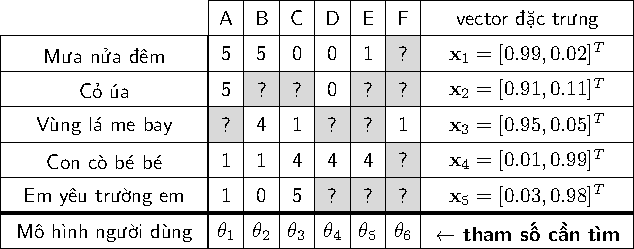
\includegraphics[width = .8 \textwidth]{Chapters/06_RecommendationSystems/23_contentbasedrecommendersys/latex/contentbased.pdf}
    \caption[]{Giả sử vector đặc trưng cho mỗi sản phẩm đã biết trước, được cho trong cột cuối
    cùng. Với mỗi người dùng, chúng ta cần tìm một mô hình \(\theta_u\) tương
    ứng.}
    \label{fig:23_2}
\end{figure}
% ****************************************************************************** 
Trong ví dụ trong Hình~\ref{fig:23_1}, chúng ta đơn giản hoá bài toán bằng việc
xây dựng một vector đặc trưng hai chiều cho mỗi bài hát: chiều thứ nhất là mức
độ \textit{Bolero}, chiều thứ hai là mức độ \textit{Thiếu nhi} của bài hát đó.
Giả sử ta đã xây dựng được vector đặc trưng cho mỗi bài hát là $\mathbf{x}_1, \mathbf{x}_2,
\mathbf{x}_3, \mathbf{x}_4, \mathbf{x}_5$ như trong Hình~\ref{fig:23_2}. Tương
tự, hành vi của mỗi người dùng cũng có thể được mô hình hoá dưới dạng tập các
tham số $\theta$. Dữ liệu huấn luyện để xây dựng mỗi mô hình $\theta_u$ là các
cặp (thông tin sản phẩm, đánh giá) tương ứng với các sản phẩm người dùng đó đã đánh giá. Việc điền giá trị còn thiếu trong ma trận
tiện ích chính là việc dự đoán mức độ quan tâm khi áp dụng mô hình $\theta_u$. Đầu ra này có thể được viết dưới dạng hàm số $f(\theta_u,
\bx_i)$. Việc lựa chọn dạng của $f(\theta_u, \bx_i)$ tuỳ thuộc vào mỗi bài toán.
Trong chương này, chúng ta sẽ quan tâm tới dạng đơn giản nhất -- dạng tuyến tính.

 
\subsection{Xây dựng hàm mất mát}
 
Đặt số lượng người dùng là $N$, số lượng sản phẩm là $M$; ma
trận thông tin sản phẩm $\bX = [\bx_1, \bx_2, \dots, \bx_M] \in\R^{d\times M}$ và ma
trận tiện ích là $\mathbf{Y} \in \R^{M \times N}$. Thành phần ở hàng thứ $m$, cột
thứ $n$ của $\mathbf{Y}$ là {mức độ quan tâm} (ở đây là số sao đã
đánh giá) của người dùng thứ $n$ lên sản phẩm thứ $m$ mà hệ thống
đã thu
thập được. Ma trận $\mathbf{Y}$ bị khuyết rất nhiều thành phần tương ứng với các
giá trị cần dự đoán. Thêm nữa, gọi $\mathbf{R}$ là ma trận thể hiện việc một người dùng đã đánh giá một
sản phẩm hay chưa. Cụ thể, $r_{mn}$ bằng một nếu sản phẩm thứ $m$ đã
được đánh giá bởi người dùng thứ $n$, bằng không trong trường hợp ngược
lại. 

\subsubsection{Mô hình tuyến tính} 
 
Giả sử ta có thể tìm được một mô hình cho mỗi người dùng, được minh hoạ
bởi một vector cột hệ số $\mathbf{w}_n \in \R^d$ và hệ số điều chỉnh $b_n$ sao cho
{mức độ quan tâm} của một người dùng tới một sản phẩm tính
được bằng một hàm tuyến tính:
\begin{equation} 
\label{eqn:23_1}
    y_{mn} = \bw_n^T\bx_m + b_n
\end{equation} 
Xét người dùng thứ $n$, nếu coi tập huấn luyện là tập hợp các
thành phần đã biết của $\mathbf{y}_n$ (cột thứ $n$ của ma
trận $\bY$), ta có thể xây dựng hàm mất
mát tương tự như hồi quy {ridge} (hồi quy tuyến tính với kiểm soát $l_2$) như sau:
\begin{equation} 
\label{eqn:23_1}
\mathcal{L}_n(\bw_n, b_n) = \frac{1}{2s_n} \sum_{m:r_{mn} = 1}(\bx_m^T\bw_n +
b_n
- y_{mn})^2
+ \frac{\lambda}{2s_n} \|\mathbf{w}_n\|_2^2
\end{equation} 
trong đó, thành phần thứ hai đóng vai trò kiểm soát và $\lambda$ là một tham số
dương; $s_n$ là số lượng các sản phẩm mà người dùng thứ $n$ đã đánh giá,
là tổng các phần tử trên cột thứ $n$ của ma trận $\mathbf{R}$, tức $s_n =
\sum_{m=1}^M r_{mn}$. Chú ý rằng cơ chế kiểm soát thường không được áp dụng lên
hệ số điều chỉnh $b_n$.
 
\index{hồi quy ridge -- ridge regression}

Vì biểu thức hàm mất mát~\eqref{eqn:23_1} chỉ phụ thuộc vào các sản phẩm đã
được đánh giá, ta có thể rút gọn nó bằng cách đặt $\hat{\mathbf{y}}_n \in
\R^{s_n}$ là
{vector con} của $\mathbf{y}_n$, được xây dựng bằng cách {trích}
các
thành phần đã biết ở cột thứ $n$ của $\bY$. Đồng thời, đặt
$\hat{\mathbf{X}}_n \in \R^{d\times s_n}$ là {ma trận con} của ma trận
đặc trưng $\mathbf{X}$, thu được bằng cách {trích} các cột tương ứng với
những sản phẩm đã được đánh giá bởi người dùng thứ $n$. Biểu thức hàm mất mát của mô hình cho người dùng thứ $n$ được viết gọn thành:
\begin{equation} 
    \mathcal{L}_n(\bw_n, b_n) = \frac{1}{2s_n}
    \|\hat{\mathbf{X}}_n^T\mathbf{w}_n + b_n
    \mathbf{e}_n- \hat{\mathbf{y}}_n\|_2^2 + \frac{\lambda}{2s_n} \|\mathbf{w}_n\|_2^2 
\end{equation} 
trong đó, $\mathbf{e}_n$ là vector cột với tất cả các thành phần bằng một. 
 Đây {chính} là hàm mất mát của hồi quy ridge. Cặp nghiệm
$\mathbf{w}_n, b_n$ có thể được tìm thông qua các thuật toán gradient
descent. Trong chương này, chúng ta sẽ trực tiếp sử dụng class
\pythoninline{Ridge} trong thư viện \pythoninline{sklearn.linear_model}. Một
điểm đáng lưu ý ở đây là $\bw_n$ chỉ được xác định nếu người dùng thứ $n$ đã
đánh giá ít nhất một sản phẩm.

% Chúng ta cùng theo dõi ví dụ nhỏ sau đây. 
 
 
\subsection{Ví dụ về hàm mất mát cho người dùng $E$ }
 
Quay trở lại ví dụ trong Hình~\ref{fig:23_2}, ma trận đặc trưng cho
các sản phẩm (mỗi cột tương ứng với một sản phẩm) là
\begin{equation} 
\bX = \bmt 
0.99 &~~ 0.91 &~~ 0.95 &~~ 0.01 &~~ 0.03 \\
0.02 &~~ 0.11 &~~ 0.05 &~~ 0.99 &~~ 0.98
\emt 
\end{equation} 
Xét trường hợp của người dùng \textit{E} với $n = 5$, $\mathbf{y}_5 = [1, ?, ?, 4,
?]^T$. Từ đó, vector nhị phân $\mathbf{r}_5 = [1, 0, 0, 1, 0]^T$. Vì \textit{E} mới chỉ
đánh giá sản phẩm thứ nhất và thứ tư nên $s_5 = 2$. Hơn nữa,
\begin{equation} 
\hat{\mathbf{X}}_5 =  
\left[\begin{matrix} 0.99 & 0.01 \\\ 0.02 & 0.99 \end{matrix} \right],
\hat{\mathbf{y}}_5 = \left[\begin{matrix} 1 \\\ 4 \end{matrix} \right], ~ \mathbf{e}_5 = \left[\begin{matrix} 1 \\\ 1 \end{matrix} \right].
\end{equation} 
Khi đó, hàm mất mát cho hệ số tương ứng với người dùng \textit{E} là:  
\begin{equation} 
\mathcal{L}_5(\bw_5, b_5) = \frac{1}{4} \left\|
\bmt 0.99 & 0.02 \\\
0.01 & 0.99 \emt\mathbf{w}_5  + b_5\bmt  1 \\\ 1 \emt -
\bmt  1 \\\ 4 \emt
\right\|_2^2 + \frac{\lambda}{4} \|\mathbf{w}_5\|_2^2 
\end{equation} 
Chúng ta sẽ áp dụng những phân tích trên đây để đi tìm nghiệm cho một bài toán gần với thực tế. 
 
 
\section{Bài toán MovieLens 100k }
 
 
\subsection{Cơ sở dữ liệu MovieLens 100k}
 
Bộ cơ sở dữ liệu MovieLens 100k (\url{https://goo.gl/BzHgtq}) được công bố năm
1998 bởi {GroupLens} (\url{https://grouplens.org}). Bộ cơ sở dữ liệu này bao gồm
100,000 (100k) đánh giá từ 943 người dùng cho 1682 bộ phim. Các bạn
cũng có
thể tìm thấy các bộ cơ sở dữ liệu tương tự với khoảng 1M, 10M, 20M đánh giá.
 
Bộ cơ sở dự liệu này bao gồm nhiều file, chúng
ta cần quan tâm các file sau:
\begin{itemize}
\item \pythoninline{u.data}: Chứa toàn bộ các đánh giá của 943 người dùng
cho 1682 bộ phim. Mỗi người dùng đánh giá ít nhất 20 bộ phim. Thông tin
về thời điểm đánh giá cũng được cho nhưng chúng ta không sử dụng trong ví dụ
này.
 
\item \pythoninline{ua.base, ua.test, ub.base, ub.test}: Là hai cách chia toàn
bộ dữ liệu ra thành hai tập con: tập huấn luyện và tập kiểm tra. Chúng ta
sẽ thực hành trên \pythoninline{ua.base} và \pythoninline{ua.test}. Bạn đọc có thể thử với cách chia dữ liệu còn lại.
 
\item \pythoninline{u.user}: Chứa thông tin về người dùng, bao gồm: id, tuổi,
giới tính, nghề nghiệp, mã vùng (zipcode). Những thông tin này có thể
ảnh hưởng tới sở thích của người dùng; tuy nhiên, chúng
ta chỉ sử dụng \textit{id} để xác định người dùng khác nhau.
 
\item \pythoninline{u.genre}: Chứa tên của 19 thể loại phim, gồm: {unknown, Action, Adventure, Animation, Children's, Comedy, Crime, Documentary, Drama, Fantasy, Film-Noir, Horror, Musical, Mystery, Romance, Sci-Fi, Thriller, War, Western,} 
 
\item \pythoninline{u.item}: Thông tin về mỗi bộ phim. Một vài dòng đầu tiên của file: 
% \newpage 
\end{itemize}
\begin{lstlisting}[language=Python]
1|Toy Story (1995)|01-Jan-1995||http://us.imdb.com/M/title-exact?Toy%20Story%20(1995)|0|0|0|1|1|1|0|0|0|0|0|0|0|0|0|0|0|0|0 
2|GoldenEye (1995)|01-Jan-1995||http://us.imdb.com/M/title-exact?GoldenEye%20(1995)|0|1|1|0|0|0|0|0|0|0|0|0|0|0|0|0|1|0|0 
3|Four Rooms (1995)|01-Jan-1995||http://us.imdb.com/M/title-exact?Four%20Rooms%20(1995)|0|0|0|0|0|0|0|0|0|0|0|0|0|0|0|0|1|0|0 
4|Get Shorty (1995)|01-Jan-1995||http://us.imdb.com/M/title-exact?Get%20Shorty%20(1995)|0|1|0|0|0|1|0|0|1|0|0|0|0|0|0|0|0|0|0 
\end{lstlisting}
Trong mỗi dòng, chúng ta sẽ thấy \textit{id} của phim, tên phim, ngày phát hành, đường dẫn và các số nhị phân \pythoninline{0}, \pythoninline{1} thể hiện bộ phim thuộc các thể loại nào trong 19 thể loại đã cho. Một bộ phim có thể thuộc nhiều thể loại khác nhau. Thông tin về thể loại này sẽ được dùng để xây dựng thông tin sản phẩm.
\newpage  
Chúng ta sử dụng thư viện
pandas (\url{http://pandas.pydata.org}) để đọc dữ liệu:

 % \pythoninline{pip install pandas}.  
 
 
\begin{lstlisting}[language=Python]
from __future__ import print_function 
import numpy as np 
import pandas as pd 
# Reading user file:
u_cols =  ['user_id', 'age', 'sex', 'occupation', 'zip_code']
users = pd.read_csv('ml-100k/u.user', sep='|', names=u_cols)
n_users = users.shape[0]
print('Number of users:', n_users)

#Reading ratings file:
r_cols = ['user_id', 'movie_id', 'rating', 'unix_timestamp']

ratings_base = pd.read_csv('ml-100k/ua.base', sep='\t', names=r_cols)
ratings_test = pd.read_csv('ml-100k/ua.test', sep='\t', names=r_cols)

rate_train = ratings_base.as_matrix()
rate_test = ratings_test.as_matrix()

print('Number of traing rates:', rate_train.shape[0])
print('Number of test rates:', rate_test.shape[0])
\end{lstlisting}
\kq
\begin{lstlisting}
Number of users: 943
Number of traing rates: 90570
Number of test rates: 9430
\end{lstlisting}
Ta sẽ chỉ quan tâm tới 19 giá trị nhị phân ở cuối mỗi hàng để xây dựng thông tin sản phẩm.
\begin{lstlisting}[language=Python]
X0 = items.as_matrix() 
X_train_counts = X0[:, -19:] 
\end{lstlisting}
 
\subsection{Xây dựng thông tin sản phẩm}
 
Công việc quan trọng trong hệ thống gợi ý dựa trên nội dung là xây dựng
vector đặc trưng cho mỗi sản phẩm. Trước hết,
chúng ta
cần lưu thông tin về các sản phẩm vào biến \pythoninline{items}:
% \newpage  
\begin{lstlisting}[language=Python]
#Reading items file:
i_cols = ['movie id', 'movie title' ,'release date','video release date', 'IMDb URL', 'unknown', 'Action', 'Adventure', 'Animation', 'Children\'s', 'Comedy', 'Crime', 'Documentary', 'Drama', 'Fantasy', 'Film-Noir', 'Horror', 'Musical', 'Mystery', 'Romance', 'Sci-Fi', 'Thriller', 'War', 'Western']

items = pd.read_csv('ml-100k/u.item', sep='|', names=i_cols) 

n_items = items.shape[0]
print('Number of items:', n_items)
\end{lstlisting}
\kq 
\begin{lstlisting}
Number of items: 1682 
\end{lstlisting}
Tiếp theo, chúng ta hiển thị một vài hàng đầu tiên của ma trận
\pythoninline{rate_train}:
\begin{lstlisting}[language=Python]
print(rate_train[:4, :])
\end{lstlisting}
\kq 
\begin{lstlisting}[language=Python]
[[        1         1         5 874965758]
 [        1         2         3 876893171]
 [        1         3         4 878542960]
 [        1         4         3 876893119]]
\end{lstlisting}
Hàng thứ nhất được hiểu là người dùng thứ nhất đánh giá bộ phim thứ
nhất năm sao. Cột cuối cùng là thời điểm đánh giá, chúng ta sẽ bỏ qua
thông số này.

Tiếp theo, chúng ta sẽ xây dựng vector đặc trưng cho mỗi sản phẩm dựa trên ma trận thể loại phim và đặc trưng {TF-IDF} (\url{https://goo.gl/bpDdQ8}) trong thư viện \pythoninline{sklearn}:
% \newpage 
\begin{lstlisting}[language=Python]
#tfidf 
from sklearn.feature_extraction.text import TfidfTransformer 
transformer = TfidfTransformer(smooth_idf=True, norm ='l2') 
X = transformer.fit_transform(X_train_counts.tolist()).toarray() 
\end{lstlisting}
 
Sau bước này, mỗi hàng của \pythoninline{X} tương ứng với vector đặc trưng của
một bộ phim.
 
\subsection{Xây dựng mô hình cho mỗi người dùng}
Với mỗi người dùng, chúng ta cần đi tìm những bộ phim nào mà
người dùng đó đã đánh giá, và giá trị của các đánh giá đó. 
% \newpage 
\begin{lstlisting}[language=Python]
def get_items_rated_by_user(rate_matrix, user_id):
    """
    return (item_ids, scores)
    """
    y = rate_matrix[:,0] # all users
    # item indices rated by user_id
    # we need to +1 to user_id since in the rate_matrix, id starts from 1 
    # but id in python starts from 0
    ids = np.where(y == user_id +1)[0] 
    item_ids = rate_matrix[ids, 1] - 1 # index starts from 0 
    scores = rate_matrix[ids, 2]
    return (item_ids, scores)
\end{lstlisting}
\
Bây giờ, ta có thể đi tìm vector trọng số của mỗi người dùng: 
 
\begin{lstlisting}[language=Python]
from sklearn.linear_model import Ridge
from sklearn import linear_model
d = X.shape[1] # data dimension
W = np.zeros((d, n_users))
b = np.zeros(n_users)
for n in range(n_users):    
    ids, scores = get_items_rated_by_user(rate_train, n)
    model = Ridge(alpha=0.01, fit_intercept  = True)
    Xhat = X[ids, :]
    model.fit(Xhat, scores) 
    W[:, n] = model.coef_
    b[n] = model.intercept_
\end{lstlisting}
 
Sau khi tính được các hệ số \pythoninline{W} và \pythoninline{b},
mức độ quan tâm của mỗi người dùng tới một bộ phim được dự đoán
bởi:
\begin{lstlisting}[language=Python]
Yhat = X.dot(W) + b 
\end{lstlisting}
 
Dưới đây là một ví dụ với người dùng có {id} bằng \pythoninline{10}:
 
% \newpage  
\begin{lstlisting}[language=Python]
n = 10
np.set_printoptions(precision=2) # 2 digits after . 
ids, scores = get_items_rated_by_user(rate_test, n)
print('Rated movies ids :', ids )
print('True ratings     :', scores)
print('Predicted ratings:', Yhat[ids, n])
\end{lstlisting}
\kq 
\begin{lstlisting}
Rated movies ids : [ 37 109 110 226 424 557 722 724 731 739]
True ratings     : [3 3 4 3 4 3 5 3 3 4]
Predicted ratings: [3.18 3.13 3.42 3.09 3.35 5.2  4.01 3.35 3.42 3.72]
\end{lstlisting}
 
\index{căn bậc hai sai số trung bình bình phương -- root mean squared error}
\index{RMSE}
\subsection{Đánh giá mô hình}
Để đánh giá mô hình tìm được, chúng ta sẽ sử dụng \textit{căn bậc hai sai số trung bình bình phương} (root mean squared error, RMSE):
\begin{lstlisting}[language=Python]
def evaluate(Yhat, rates, W, b):
    se = cnt = 0
    for n in xrange(n_users):
        ids, scores_truth = get_items_rated_by_user(rates, n)
        scores_pred = Yhat[ids, n]
        e = scores_truth - scores_pred 
        se += (e*e).sum(axis = 0)
        cnt += e.size 
    return np.sqrt(se/cnt)

print('RMSE for training: %.2f' %evaluate(Yhat, rate_train, W, b))
print('RMSE for test    : %.2f' %evaluate(Yhat, rate_test, W, b))
\end{lstlisting}
\kq 
\begin{lstlisting}
RMSE for training: 0.91
RMSE for test    : 1.27
\end{lstlisting}
 
 
Như vậy, với training set, sai số vào khoảng 0.91 (sao); với test set, sai số
lớn hơn một chút, khoảng 1.27. Các kết quả này chưa thực sự tốt
vì mô hình đã được đơn giản hoá quá nhiều. Kết quả tốt hơn có thể được thấy
trong các chương tiếp theo về lọc cộng tác. 
 
 
\section{Thảo luận}

\begin{itemize}
    \item Hệ thống gợi ý dựa trên nội dung là một phương pháp gợi ý đơn giản. Đặc điểm của phương pháp này là việc xây dựng mô hình cho mỗi người dùng không phụ thuộc vào người dùng khác.  
     
    \item Việc xây dựng mô hình cho mỗi người dùng có thể coi như bài
    toán hồi quy với dữ liệu huấn luyện là thông tin sản phẩm và đáng giá của người dùng đó về sản phẩm đó. Thông tin sản phẩm không phụ thuộc vào người dùng mà phụ thuộc vào các đặc điểm mô tả của sản phẩm.
     
    \item Mã nguồn trong chương này có thể tìm thấy tại
    \url{https://goo.gl/u9M3vb}.
\end{itemize}
 
 
 
\textbf{Đọc thêm}
\begin{enumerate}
    \item \textit{Recommendation Systems -- Stanford InfoLab}
    (\url{https://goo.gl/P1pesC}).

    \item \textit{Recommendation systems -- Machine Learning, Andrew Ng}
    (\url{https://goo.gl/jdFvej}).


    \item \textit{Content Based Recommendations -- Stanford University}
    (\url{https://goo.gl/3wnbZ4}).
\end{enumerate}
